\documentclass[12pt, a4paper]{article}

\usepackage[english]{babel}
\usepackage[T1]{fontenc}
\usepackage[utf8]{inputenc}
\usepackage{amsmath}
\usepackage{graphicx}
\usepackage[section]{placeins}
\usepackage{listings}
\usepackage{tabularx}
\usepackage{booktabs}
\usepackage{tcolorbox}
\usepackage[a4paper,margin=1in]{geometry}
\usepackage{float}
\usepackage{fontawesome5}
\usepackage{xcolor}
\usepackage{hyperref}
\hypersetup{
  colorlinks=true,
  urlcolor=blue!55!black,
  linkcolor=black,
  citecolor=black,
}

\setlength{\textheight}{24cm}
\setlength{\textwidth}{15cm}
\setlength{\footskip}{5mm}
\setlength{\oddsidemargin}{0mm}
\setlength{\evensidemargin}{0mm}
\setlength{\topmargin}{0mm}
\setlength{\headsep}{0mm}

% ---------- shell listings ----------
\definecolor{shellbg}{RGB}{245,246,248}
\definecolor{shellframe}{RGB}{200,205,212}
\definecolor{shellcomment}{RGB}{110,120,130}
\lstdefinestyle{shell}{
  language=bash,
  basicstyle=\ttfamily\small,
  backgroundcolor=\color{shellbg},
  frame=single,
  rulecolor=\color{shellframe},
  framesep=4pt,
  xleftmargin=6pt,
  xrightmargin=6pt,
  breaklines=true,
  breakatwhitespace=false,
  columns=fullflexible,
  keepspaces=true,
  showstringspaces=false,
  commentstyle=\color{shellcomment}\itshape,
  keywordstyle=\color{black},
}
\lstset{style=shell}

% ---------- important box ----------
\newtcolorbox{important}{colback=orange!6, colframe=orange!70!black,
  boxrule=0.6pt, arc=2pt, left=6pt, right=6pt, top=4pt, bottom=4pt,
  fonttitle=\bfseries, title=Important}
\lstdefinelanguage{json5}{
  morestring=[b]",
  morecomment=[l]{//},
}


% Figure that falls back to a framed placeholder when the image is missing
\newcommand{\figimg}[3]{%
  \begin{figure}[H]
    \centering
    \IfFileExists{#1}{%
      \includegraphics[width=#2\textwidth]{#1}%
    }{%
      \fbox{\parbox[c][4cm][c]{#2\textwidth}{\centering\small\ttfamily missing: #1}}%
    }
    \caption{#3}
    \label{fig:#1}
  \end{figure}%
}

\begin{document}

% ===== Title page =====
\begin{titlepage}
\centering

\includegraphics[width=0.9\textwidth]{img/logo_AGH.jpg}\\[1.5cm]

\vspace{1.0cm}

{\LARGE\bfseries Distance Measurements with the use of\\
 Millimeter-Wave Radars\par}
\vspace{8pt}
{\Large Setup and User Guide\par}
\vspace{2.5cm}

{\large Bartłomiej Woś\par}
{\large November 2026\par}
\end{titlepage}

\newpage
\tableofcontents


\newpage
\section{Introduction}
This document provides a brief guide to running the data-acquisition software
for the TI IWR1843BOOST radar evaluation board developed as part of a master's thesis, as well as
to building and potentially extending the existing software modules. The following
sections present a step-by-step tutorial covering, respectively:

\begin{itemize}
  \item building and flashing the firmware onto the IWR1843 device
  \item building the Python application for radar configuration and data acquisition
  \item offline post-processing in MATLAB
\end{itemize}

The tutorial is based on the project file structure available in the public
repository:
\begin{center}
\faGithub~\href{https://github.com/BartlomiejWos/Distance-Measurment-Using-mmWave-Radars}
            {\texttt{github.com/BartlomiejWos/Distance-Measurment-Using-mmWave-Radars}}
\end{center}

\begin{lstlisting}
git clone https://github.com/BartlomiejWos/Distance-Measurment-Using-mmWave-Radars.git
cd Distance-Measurment-Using-mmWave-Radars
\end{lstlisting}
 
\medskip
\noindent\textbf{Note:} The IWR1843BOOST board used in the project was flashed with the modified firmware
described in Section~\ref{sec:firmware}, which is required by the acquisition application.
To use the TI web interface (mmWave Demo Visualizer,
\url{https://dev.ti.com/gallery/view/mmwave/mmWave_Demo_Visualizer/}), flash the
precompiled TI out-of-box demo instead (procedure in Section~\ref{sec:flash}):
\begin{lstlisting}
radar_firmware/precompiled_binaries/xwr18xx_mmw_demo.bin
\end{lstlisting}
The same binary is part of the TI mmWave SDK (link in Section \ref{sec:firmware} and can also be downloaded from the TI
website.





\newpage
\section{Firmware}
\label{sec:firmware}

The custom MSS firmware is based on the TI mmWave Studio CLI firmware and extends it
to support up to 512 unique chirps per frame, which is required for the SFCW emulation.

The IWR1843BOOST board used in the project is already flashed (or should be) with the custom firmware.
If no changes to the firmware are planned, this section can be skipped and you can go
directly to Section~\ref{sec:app}. If the firmware has to be modified, follow the steps
below to build the new binary and flash it onto the board.

\subsection{Requirements}
To build the firmware locally, install the tools listed in the table below.
Note that the XDS110 drivers are necessary for proper UART communication with the IWR1843 device.
\begin{table}[H]
\centering
\caption{Firmware build and flashing tools.}
\begin{tabularx}{\textwidth}{|l|X|}
\hline
\textbf{Tool} & \textbf{Used for} \\
\hline
Code Composer Studio (CCS) & Firmware build IDE \\
\hline
TI mmWave SDK 3.6.2 LTS & Firmware libraries and drivers, RadarSS firmware, binary-creation tools \\
\hline
UniFlash & Flashing the firmware binary \\
\hline
XDS110 drivers & USB/UART connection to the IWR1843BOOST (installed with CCS or UniFlash) \\
\hline
\end{tabularx}
\end{table}

\noindent
Useful links:
\begin{itemize}
  \item CCS: \url{https://www.ti.com/tool/CCSTUDIO}
  \item mmWave SDK: \url{https://www.ti.com/tool/MMWAVE-SDK}
  \item UniFlash: \url{https://www.ti.com/tool/UNIFLASH}
  \item XDS110 Windows drivers (XDS Emulation Software Package): \url{https://software-dl.ti.com/ccs/esd/documents/xdsdebugprobes/emu_xds_software_package_download.html}
  \item Radar Toolbox (original Studio CLI project): \url{https://www.ti.com/tool/RADAR-TOOLBOX}
\end{itemize}

\subsection{Building}

\begin{enumerate}
  \item Install the mmWave SDK and CCS. The SDK installer also installs SYS/BIOS,
        XDCtools and the ARM compiler in the versions required by the project.
  \item Start CCS and Import the project: \textbf{File $\rightarrow$ Import $\rightarrow$ Projects}
  \item Browse to: \texttt{radar\_firmware/1843/} and select
        \texttt{studio\_cli\_xwr18xx.projectspec}. The original, unmodified TI project is
        available in the TI Radar Toolbox:\\
        \texttt{<radar\_toolbox\_install\_dir>/tools/studio\_cli/src/1843/}.
  \item Build: \textbf{Project $\rightarrow$ Build All}.
\end{enumerate}


\begin{figure}[H]
\centering
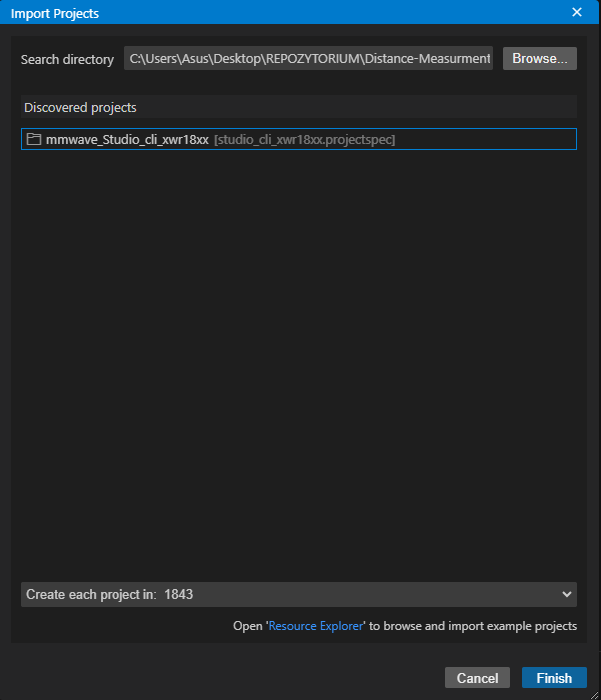
\includegraphics[width=0.75 \textwidth]{img/ccs.png}
\caption{Importing the project specification in CCS.}
\label{fig:ccs_import}
\end{figure}


\begin{figure}[H]
\centering
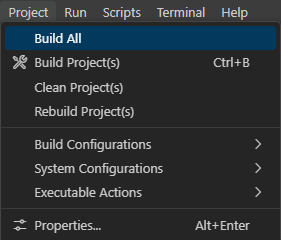
\includegraphics[width=0.4\textwidth]{img/ccs_2.png}
\caption{Building the imported project.}
\label{fig:ccs_import}
\end{figure}

The resulting binary is located in the \texttt{Debug} folder of the CCS project:
\begin{lstlisting}
<workspace>/mmwave_Studio_cli_xwr18xx/Debug/mmwave_Studio_cli_xwr18xx.bin
\end{lstlisting}

\subsection{Flashing}
\label{sec:flash}

The boot mode of the IWR1843 is selected by the Sense-On-Power (SOP) jumpers on the
IWR1843BOOST board (Fig.~\ref{fig:soop}).

\begin{table}[H]
\centering
\caption{SOP switch settings.}
\begin{tabular}{|l|c|c|c|}
\hline
\textbf{Mode} & \textbf{SOP2} & \textbf{SOP1} & \textbf{SOP0} \\
\hline
Flashing   & ON  & OFF & ON \\
\hline
Functional & OFF & OFF & ON \\
\hline
\end{tabular}
\end{table}

\begin{figure}[H]
\centering
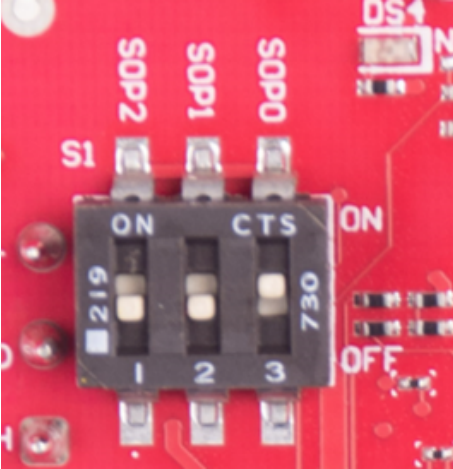
\includegraphics[width=0.4\textwidth]{img/sop_jumpers.png}
\caption{SOP jumpers on the IWR1843BOOST}
\label{fig:soop}
\end{figure}

To flash the binary, set the board to flashing mode and use UniFlash as described in the
TI flashing guide:\\
\url{https://dev.ti.com/tirex/explore/node?node=A__AQGDCdbNj-0pSybFx0P7GQ__radar_toolbox__1AslXXD__LATEST}


\begin{important}
The board must be in functional mode during measurements. Otherwise, the device waits for
a new binary after every reset.
\end{important}


\newpage
\section{Python application}
\label{sec:app}

The host application (\texttt{radar\_app}) configures the radar over UART and controls the DCA1000EVM over Ethernet.
Communication with the DCA1000 FPGA is implemented by the C++ extension module \texttt{radar\_api.pyd}, built with PyBind11
on top of the TI \texttt{RF\_API} library. Since this module has to be compiled and the application is packaged into a single
executable, the whole project is built with the MSYS2 MinGW64 toolchain.

\subsection{Requirements}

\begin{table}[H]
\caption{Host application environment requirements.}
\centering
\begin{tabularx}{\textwidth}{|l|X|}
\hline
\textbf{Tool} & \textbf{Used for} \\
\hline
MSYS2 (MinGW64) & GCC, make, Python 3.14, PyInstaller \\
\hline
PyBind11 & C++ / Python bindings of the DCA1000 module \\
\hline
XDS110 drivers & UART connection to the radar (installed with CCS or UniFlash, see Section~\ref{sec:firmware}) \\
\hline
\end{tabularx}
\end{table}

All of them are installed in the MSYS2 shell as described below.

\subsection{Environment and build tools}

\subsubsection{MSYS2}

Install MSYS2 from \url{https://www.msys2.org}, open the \textbf{MSYS2 MINGW64} shell and
set up the build tools and Python:
\begin{lstlisting}
pacman -Syu
pacman -S --needed git make mingw-w64-x86_64-gcc
pacman -S --needed mingw-w64-x86_64-python mingw-w64-x86_64-python-pip
python --version
\end{lstlisting}

\subsubsection{PyBind11}

Install PyBind11 in the same shell:
\begin{lstlisting}
pacman -S --needed mingw-w64-x86_64-pybind11
\end{lstlisting}

\subsubsection{DCA1000 module}

Build the extension module:
\begin{lstlisting}
cd radar_app/src/libs/dca1000
make
\end{lstlisting}

\newpage
\noindent
The compiled module is written to:
\begin{lstlisting}
radar_app/src/hwctl/dca1000/radar_api.pyd
\end{lstlisting}

\noindent
The TI libraries \texttt{RF\_API.dll} and \texttt{ReleaseRF\_API.dll} are loaded at
runtime from:
\begin{lstlisting}
radar_app/src/libs/dca1000/ti-external/
\end{lstlisting}


\begin{important}
The \texttt{Makefile} is set up for Python 3.14. If MSYS2 installed a different version,
pass it on the command line, e.g.\ \texttt{make PYTHON\_VERSION=3.13}.
A \texttt{.pyd} built for one Python version cannot be imported by another.
\end{important}


\subsubsection{Python packages}

From the root of the repository, install the application requirements and PyInstaller:
\begin{lstlisting}
pip install --break-system-packages -r radar_app/requirements.txt
\end{lstlisting}
\texttt{--break-system-packages} is required because MSYS2 marks its Python as
externally managed.


\subsubsection{Building the executable}
Package the application into a single \texttt{radar\_app.exe}:
\begin{lstlisting}
cd radar_app
./scripts/build.sh
\end{lstlisting}

The executable is written to \texttt{radar\_app/build/dist/} and runs from any shell,
without MSYS2.

\begin{important}
Run \texttt{build.sh} from the MinGW64 shell. An executable built with a different Python
cannot load \texttt{radar\_api.pyd}.
\end{important}


\subsubsection{Code checks (optional)}
Install the static type checker and linter:
\begin{lstlisting}
pacman -S --needed mingw-w64-x86_64-mypy mingw-w64-x86_64-python-flake8
\end{lstlisting}

Run the checks:
\begin{lstlisting}
cd radar_app
./scripts/checkstyle.sh
\end{lstlisting}




\newpage
\subsection{Network configuration}

The DCA1000EVM uses a fixed IP configuration. The PC Ethernet adapter connected to
the DCA1000 must have a static address:

\begin{table}[H]
\centering
\caption{DCA1000 network settings.}
\begin{tabular}{|l|l|}
\hline
PC IP address & \texttt{192.168.33.30} \\
\hline
Subnet mask & \texttt{255.255.255.0} \\
\hline
DCA1000 IP address & \texttt{192.168.33.180} \\
\hline
Config / data UDP ports & \texttt{4096} / \texttt{4098} \\
\hline
\end{tabular}
\end{table}

\begin{important}
Disable the Windows firewall for this network.
Otherwise the PC does not receive data from the DCA1000 and the capture hangs.
\end{important}



\subsection{Configuration file}

The radar is configured with a \texttt{.json5} file. Two examples are provided:
\path{radar_app/src/cfg_fmcw.json5} and \path{radar_app/src/cfg_sfcw.json5}.
Before the first run, set the COM port of the radar and the output directory:

\begin{lstlisting}[language=json5]
{
output_path: "C:\\data\\measurements",   // captures are stored here
com_port: "COM22",                       // XDS110 Application/User UART
...
}
\end{lstlisting}

\noindent
The remaining parameters are translated into the firmware CLI commands\\
(\texttt{channelCfg}, \texttt{adcCfg}, \texttt{profileCfg}, \texttt{chirpCfg},
\texttt{frameCfg}). Their meaning is described in the mmWave SDK User Guide:\\
\url{https://software-dl.ti.com/ra-processors/esd/MMWAVE-SDK/latest/exports/mmwave_sdk_user_guide.pdf}
\noindent
Some parameters are not exposed in the configuration file and are set in the code, e.g.\ the 16-bit ADC resolution, chirp indices and LVDS stream settings.


\subsubsection{Running the application}

From source, in the MSYS2 MinGW64 shell:
\begin{lstlisting}
cd radar_app/src
python entrypoint.py --cfg-file-path cfg_fmcw.json5 --file-prefix <test>
\end{lstlisting}

\noindent
As an executable, from any shell:
\begin{lstlisting}
radar_app.exe --cfg-file-path cfg_sfcw.json5 --auto-prefix <meas>
\end{lstlisting}

\begin{table}[H]
\centering
\begin{tabularx}{\textwidth}{|l|X|}
\hline
\textbf{Argument} & \textbf{Description} \\
\hline
\texttt{--cfg-file-path} & path to the \texttt{.json5} configuration \\
\hline
\texttt{--file-prefix NAME} & name of the capture folder \\
\hline
\texttt{--auto-prefix BASE} & auto-incremented recording: \texttt{BASE\_000}, \texttt{BASE\_001}, \ldots \\
\hline
\texttt{-v} & enable DEBUG logging \\
\hline
\end{tabularx}
\caption{Command-line arguments.}
\end{table}




Each capture is stored in its own folder \texttt{<output\_path>/<prefix>/}.

\begin{figure}[H]
\centering
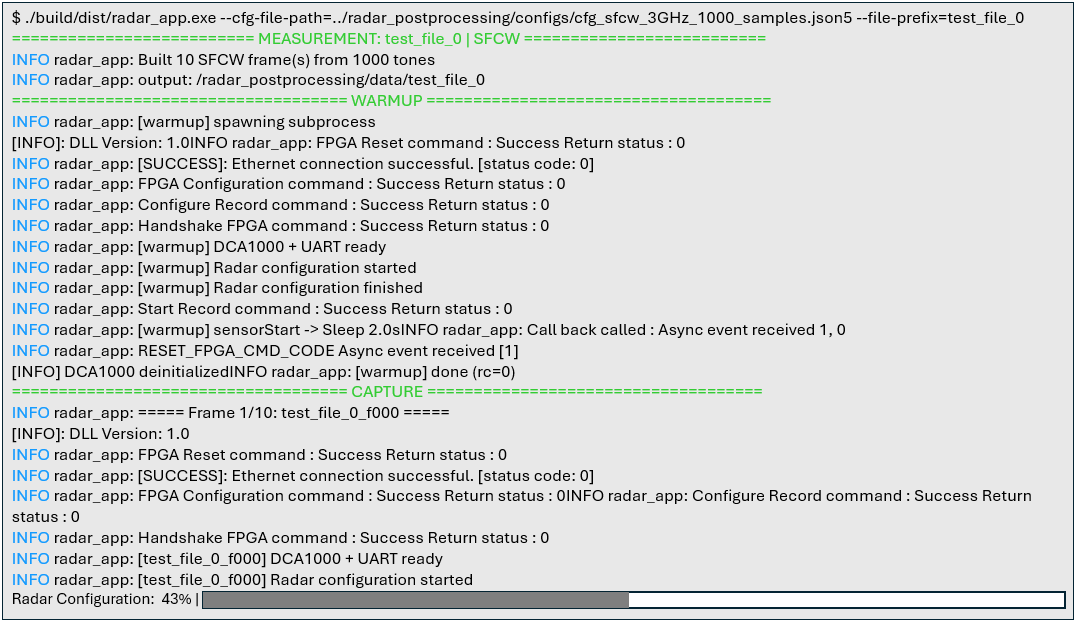
\includegraphics[width=1.0\textwidth]{img/app_photo.png}
\caption{Application log output.}
\label{fig:connection}
\end{figure}


The application must be started from \texttt{radar\_app/src}, because it re-launches
itself for every frame with \texttt{python -m entrypoint}. Use an absolute
\texttt{output\_path} to avoid captures being stored relative to the working directory.

\medskip
\noindent\textbf{Note:}\\
When the application is started by the robot motion software,
pass the path to \texttt{radar\_app.exe} without any arguments. It then runs with the
default configuration defined in \path{radar_app/src/cfg/default.py} and auto-incremented
recordings (\texttt{meas\_000}, \texttt{meas\_001}, \ldots). Check this file before the
measurements and set \texttt{output\_path} and \texttt{com\_port} for the PC in use.
To switch between FMCW and SFCW, set \texttt{DEFAULT\_CFG} in this file and rebuild the
executable.





\newpage
\section{Connection and board settings}

Fig.~\ref{fig:connection} shows the connections between the PC and the boards. The radar is
configured over UART, and the raw ADC data is streamed by the DCA1000EVM over Ethernet.

\begin{figure}[H]
\centering
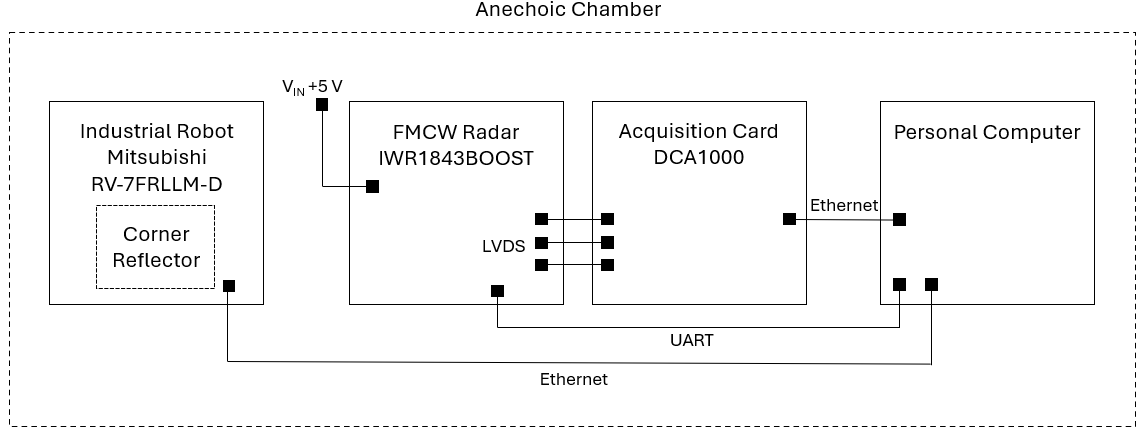
\includegraphics[width=1.0\textwidth]{img/meas_schem.png}
\caption{Connection diagram.}
\label{fig:connection}
\end{figure}

The DIP switch settings of the DCA1000EVM and the raw data capture are described in the
TI documentation (the eval board used in the project should already be set correctly):
\begin{itemize}
\item DCA1000EVM Data Capture Card User's Guide: \url{https://www.ti.com/lit/pdf/spruij4}
\item mmWave Radar Device ADC Raw Data Capture: \url{https://www.ti.com/lit/pdf/swra581}
\end{itemize}



\newpage
\section{Post-processing}

The post-processing is implemented in MATLAB in \path{radar_postprocessing/core/}.
Every script has a configuration block at the top (data folder, capture prefix, enabled corrections etc.),
which can be adjusted before running.

\subsection{Measurement data}

The measurements used in the thesis are stored in
\path{radar_postprocessing/measurement_data/}:
\begin{itemize}
\item \path{fmcw_sweep/}: 75 FMCW captures (\texttt{fmcw\_comparision\_000} \ldots\ \texttt{074}),
\item \path{sfcw_sweep/}: 75 SFCW captures (\texttt{sfcw\_comparision\_000} \ldots\ \texttt{074}).
\end{itemize}
Each capture corresponds to one robot position and contains
the raw DCA1000 files (\texttt{*\_Raw\_0.bin}) and \texttt{metadata.json} with the radar
configuration. All scripts point to this folder by default, so they can be run directly
after cloning the repository.

\subsection{Scripts}

\begin{table}[H]
\centering
\begin{tabularx}{\textwidth}{|l|X|}
\hline
\textbf{Script} & \textbf{Purpose} \\
\hline
\texttt{fmcw/run\_fmcw.m} & range profile of a single FMCW capture \\
\hline
\texttt{sfcw/run\_sfcw.m} & range profile of a single SFCW capture \\
\hline
\texttt{sfcw/calibration/run\_sfcw\_calib.m} & SFCW calibration; saves \texttt{sfcw\_calibration.mat} in the same folder \\
\hline
\texttt{fmcw/fmcw\_displacement\_analysis.m} & FMCW displacement tracking  \\
\hline
\texttt{sfcw/sfcw\_displacement\_analysis.m} & SFCW displacement tracking  \\
\hline
\texttt{analysis/fmcw\_sfcw\_coarse\_fine\_plots.m} & combined result plots \\
\hline
\end{tabularx}
\caption{Main MATLAB scripts.}
\end{table}

Recommended order:
\begin{enumerate}
\item add \path{radar_postprocessing/} to the MATLAB path;
\item check single captures with \texttt{run\_fmcw.m} / \texttt{run\_sfcw.m};
\item for SFCW, run \texttt{run\_sfcw\_calib.m} to create the calibration file;
\item run \texttt{fmcw\_displacement\_analysis.m} and \texttt{sfcw\_displacement\_analysis.m};
      the results are saved to \path{analysis/cmp_fmcw_displacement.mat} and
      \path{analysis/cmp_sfcw_displacement.mat};
\item compare both modes with the scripts in \texttt{analysis/}.
\end{enumerate}

Scripts add the required helper folders (\texttt{common/parser}, \texttt{common/utils\_dsp})
to the MATLAB path automatically, so they can be run directly from the editor.

\end{document}
